\section{(Des)estructura secundaria de prote\'\i{}nas} \label{protSS}

La estructura secundaria es una propiedad de las prote\'\i{}nas naturales en soluci\'{o}n, 
que se explica por medio de una red (din\'{a}mica) de puentes de hidr\'{o}geno que conectan diferentes partes del polip\'{e}ptido 
a escala m\'{a}s o menos local, formando h\'{e}lices y l\'{a}minas que quedan conectadas por lazos (\italics{loops}) y regiones 
desordenadas, como ya recordamos en la secci\'{o}n \ref{SS} 
(y en este \htmladdnormallink{otro curso}{http://www.eead.csic.es/compbio/material/modelado_comparativo/node5.html}). 

Si disponemos de las coordenadas at\'{o}micas de una prote\'{i}na podemos medir sus \'{a}ngulos diedros 
para generar nuestros propios diagramas de Ramachandran, como hace 
\htmladdnormallink{esta herramienta web}{http://dicsoft1.physics.iisc.ernet.in/rp/}, con dos fines:
\begin{itemize}
\item Comprobar qu\'{e} residuos de la secuencia se encuentran en conformaciones (regiones) favorables, como medida de calidad
de la estructura. 
\item Averiguar en base a la geometr\'{i}a del esqueleto proteico el estado de estructura secundaria de segmentos de residuos
(como en este \htmladdnormallink{ejercicio}{http://www.eead.csic.es/compbio/material/bioperl/node53.html}). 
\end{itemize}

El procedimiento, dado unas coordenadas en formato PDB (\htmladdnormallink{1LFU}{./files/1lfu.html}),
es relativamente sencillo, recurriendo a programas como \htmladdnormallink{DANGLE}{http://kinemage.biochem.duke.edu/software/dangle.php}
o haciendo un poco de \'{a}lgebra y trigonometr\'{i}a:
\verbatiminput{code/prog2.2.pl}

\begin{figure}
\begin{center} 
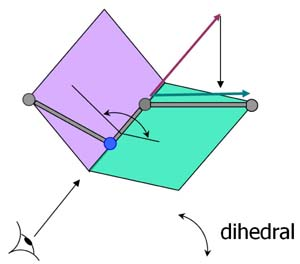
\includegraphics{signo_diedro1}
\caption%[fi y psi en el esqueleto pept?dico]
{
Definici\'{o}n de \'{a}ngulo diedro, 
figura tomada de \htmladdnormallink{http://structuralbioinformatics.com}{http://structuralbioinformatics.com}.
}
\label{fig:signo_diedro1}
\end{center}
\end{figure}

%\begin{figure}
%\begin{center} 
%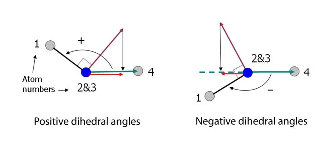
\includegraphics{signo_diedro2}
%\caption%[fi y psi en el esqueleto pept?dico]
%{
%Signo de un \'{a}ngulo diedro, 
%figura tomada de \htmladdnormallink{http://structuralbioinformatics.com}{http://structuralbioinformatics.com}.
%}
%\label{fig:signo_diedro2}
%\end{center}
%\end{figure}

Otras definiciones de estructura secundaria se basan en encontrar patrones de puentes de 
hidr\'{o}geno entre grupos $-CO$ y $-NH$ del esqueleto pept\'{i}dico, 
como por ejemplo hace el software \htmladdnormallink{DSSP}{http://swift.cmbi.ru.nl/gv/dssp/} \citep{Kabsch1983}
de acuerdo con esta definici\'{o}n energ\'{e}tica, donde un puente v\'{a}lido debe tener $E<-0{.}5 kcal/mol$, 
$q_{1}=0.42e$, $q_{2}=0.20e$ y $r$ es una distancia interat\'{o}mica en Angstroms:
\begin{equation}
E = q_{1} q_{2} \left[ \frac{1}{r_{ON}} + \frac{1}{r_{CH}} - \frac{1}{r_{OH}} - \frac{1}{r_{CN}} \right] \cdot 332 \ \mathrm{kcal/mol}
\label{eq:dssp}
\end{equation}

El software \htmladdnormallink{STRIDE}{http://webclu.bio.wzw.tum.de/stride/} \citep{Frishman1995} es otro programa para este fin 
que en experimentos de validaci\'{o}n mejora las asignaciones de estructura secundaria de DSSP.

Sin embargo, frecuentemente el problema es todav\'{i}a m\'{a}s complicado:
\begin{itemize}
\item \textbf{PROBLEMA:} tenemos una secuencia proteica pero no conocemos su estructura 
\item \textbf{SOLUCI\'{O}N PROPUESTA:} reconocer en la secuencia segmentos que formen h\'{e}lices y l\'{a}minas, y lazos 
para caracterizar su topolog\'{i}a o estructura secundaria 
\end{itemize} 

Si calculamos alineamientos m\'{u}ltiples de secuencias de prote\'{i}nas hom\'{o}logas,
las columnas del alineamiento resultante permiten deducir patrones de sustituci\'{o}n de amino\'{a}cidos
que son espec\'{i}ficos de posici\'{o}n. Esta fuente de informaci\'{o}n evolutiva,
combinada con algoritmos basados en \htmladdnormallink{redes neuronales}{https://en.wikipedia.org/wiki/Artificial_neural_network},
permite predecir con una precisi\'{o}n cercana al 75\% la estructura secundaria en 3 estados (H=h\'{e}lice alfa, E=l\'{a}mina beta y C=coil).
Es evidente que se pierde informaci\'{o}n con este alfabeto, pero la estructura inferida puede tener muchas aplicaciones a la hora de dise\~nar 
experimentos y algoritmos que trabajen sobre la estructura terciaria. 

Hay una buena exposici\'{o}n de este tema en el art\'\i{}culo de \cite{Jones1999}, 
donde se presenta el algoritmo \htmladdnormallink{PSIPRED}{http://bioinf.cs.ucl.ac.uk/psipred}
y se eval\'{u}a la precisi\'{o}n de las asignaciones de estructura secundaria de varias maneras, incluyendo la funci\'{o}n:
\begin{equation}
Q_{3} = \frac{\sum\limits_{i=H,E,C}{corrpred_{i}}}{\sum\limits_{i=H,E,C}{obs_{i}}} \times 100
\end{equation}

En \citet{Jurtz2017} se explica en mayor detalle c\'{o}mo funcionan este tipo de predictores, 
incluyendo \htmladdnormallink{c\'{o}digo fuente en python2.7}{https://github.com/vanessajurtz/lasagne4bio}
para programar uno.

%\begin{equation}
%Sov = \frac{1}{N} \sum_{s}\frac{minsolap (s_{obs},s_{pred})}{maxsolap (s_{obs},s_{pred})} \times 100)
%\end{equation}

\begin{figure}
\begin{center} 
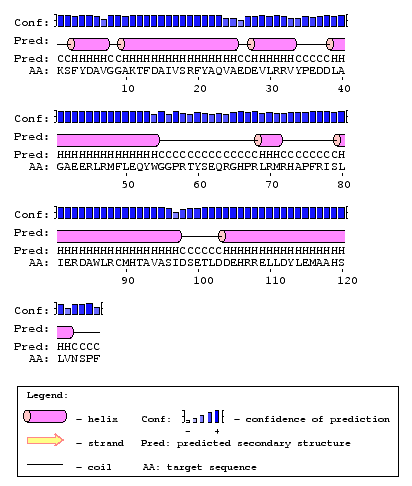
\includegraphics{ss1}
\caption%[]
{
Ejemplo de predicci\'{o}n de estructura secundaria de PSIPRED, 
obtenida en el servidor \htmladdnormallink{PSIPRED}{http://bioinf.cs.ucl.ac.uk/psipred}.
}
\label{fig:psipred}
\end{center}
\end{figure}

PSIPRED es aceptado como uno de los mejores predictores, pero hay muchos otros algoritmos de predicci\'{o}n de estructura secundaria y 
la mejor manera de compararlos es por medio de evaluaciones autom\'{a}ticas a ciegas. Desgraciadamente, este tipo de iniciativas, como  
\htmladdnormallink{LiveBench}{http://en.wikipedia.org/wiki/LiveBench} o EVA,  
que recolectan datos de distintos algoritmos a medida que crece el PDB, son financiadas por poco tiempo y mueren.

Tras la aparici\'{o}n de los primeros predictores de estructura secundaria empez\'{o} a ser evidente que muchas prote\'{i}nas, 
sobre todo de vertebrados, no ten\'{i}an aparentemente una estructura ordenada, al menos en ciertos estados fisiol\'{o}gicos 
(ver por ejemplo el repositorio \htmladdnormallink{Disprot}{http://www.disprot.org} \citep{Sickmeier2007,yruela_inmaculada_2014_1066352}).
Hoy sabemos que muchas prote\'{i}nas ordenadas pueden contener segmentos desordenados o d\'{u}ctiles \citep{Lobanov2010}.
Como resultado se dise\~naron predictores para un cuarto estado, el de desorden intr\'{i}nseco, y se han creado recursos para la 
anotaci\'{o}n de estas secuencias como \htmladdnormallink{D2P2}{http://d2p2.pro}.

En el caso de PSIPRED, la evoluci\'{o}n es un software de nombre
\htmladdnormallink{DISOPRED}{http://bioinfadmin.cs.ucl.ac.uk/downloads/DISOPRED} \citep{Ward2004},
que adem\'{a}s de reconocer elementos de estructura secundaria estima la probabilidad de que cada residuo est\'{e} desordenado,
sin pertenecer a ninguna clase de estructura secundaria.

La mayor\'{i}a de predictores de estructura secundaria y desorden tienen mejores resultados cuando
extraen informaci\'{o}n evolutiva de secuencias hom\'{o}logas. Sin embargo, esto implica que 
estos algoritmos son sensibles al contenido de las bases de datos de secuencias p\'{u}blicas, 
como se muestra en la siguiente figura:

\begin{figure}
\begin{center} 
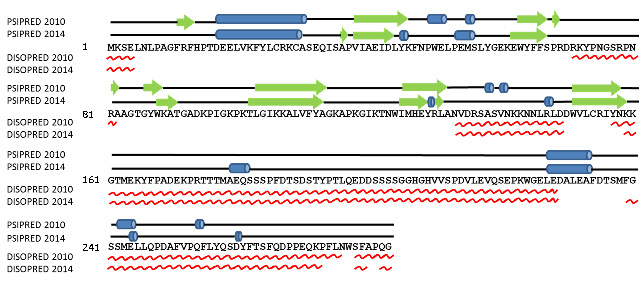
\includegraphics{disopredTime2}
\caption%[]
{
Comparaci\'{o}n de predicciones de PSIPRED (estructura secundaria) y DISOPRED2 (desorden) 
para la secuencia NAC81 de Arabidopsis thaliana calculadas sobre versiones de 2010 y 2014 
de la colecci\'{o}n de secuencias \htmladdnormallink{uniref90}{https://www.uniprot.org/help/uniref}.
Se marcan en rojo los segmentos desordenados, las h\'{e}lices en azul y las l\'{a}minas $\beta$ en verde.
Figura de \citet{Yruela2014}.
}
\label{fig:disopredTime}
\end{center}
\end{figure}

%\begin{figure}
%\begin{center} 
%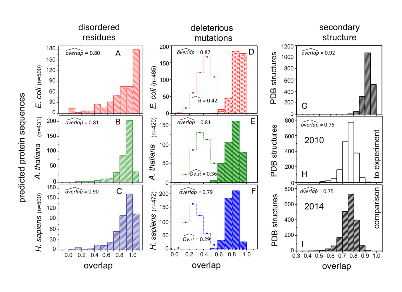
\includegraphics{disopredTime}
%\caption%[]
%{
%Consistency of intrinsically disordered residues predicted by DISOPRED2 (A, B ,C), 
%amino acid substitutions affecting function predicted by SIFT (D, E, F), 
%and PSIPRED secondary structure predictions (G). 
%Sets of proteins from E. coli (red), A. thaliana (green) and H. sapiens (blue), 
%as well as a collection of high quality PDB structures (grey, n=1983) 
%were analyzed using uniref90 database snapshots from 2010 and 2014 and their overlap computed as explained in Methods. 
%For SIFT two kinds of histograms are produced, using the strict (dashed line) and set-based (solid columns) overlap functions. 
%Panels H and I benchmark the quality of 2010 and 2014 secondary structure predictions by showing the overlap of PSIPRED 
%results and experimentally determined protein structures. 
%}
%\label{fig:disopred1}
%\end{center}
%\end{figure}

Otros predictores que combinan estructura secundaria y otras propiedades son 
\htmladdnormallink{s2D}{http://www-mvsoftware.ch.cam.ac.uk/} o 
\htmladdnormallink{SPIDER2}{http://sparks-lab.org/server/SPIDER2}, con una precisi\'{o}n por encima del 80\% \citep{Sormanni2014,Heffernan2015},
o \htmladdnormallink{SSpro}{http://scratch.proteomics.ics.uci.edu/}, rayando el \%90 en las validaciones de sus autores \citep{Magnan2014}.
Probablemente se alcanzado ya el techo para predicciones de 3 estados, pero queda espacio para mejorar las predicciones 
de los 8 estados de DSSP \citep{Yang2018}. % (ver tabla \ref{tab:SS8}).

De acuerdo con meta-an\'{a}lisis recientes los mejores predictores de desorden son
\htmladdnormallink{DISOPRED}{http://bioinf.cs.ucl.ac.uk/psipred/?disopred=1},
\htmladdnormallink{PrDOS}{http://prdos.hgc.jp/cgi-bin/top.cgi} y
\htmladdnormallink{AUCpreD}{http://raptorx2.uchicago.edu/StructurePropertyPred/predict}
\citep{Wang2016,Meng2017}

El ejercicio de esta secci\'{o}n consiste en calcular la estructura secundaria de una prote\'\i{}na del 
\htmladdnormallink{Protein Data Bank}{http://www.rcsb.org/pdb} de 3 maneras distintas, con el fin de compararlas:
\begin{itemize}
\item por medio de PSIPRED, que en realidad es un predictor,
\item modificando el programa prog2.2.pl, calculando segmentos de secuencia que tengan el mismo estado de estructura secundaria
seg\'{u}n el diagrama de Ramachandran y 
\item por medio del programa STRIDE, simplificando segmentos de estructura secundaria (H=G,H,I; E=E,B y C=resto de estados)
\item alinea las estructuras secundarias en alfabeto simplificado de tres letras y describe las diferencias observadas
\item (los ejecutables necesarios se encuentran en \verb+/home/compu2/algoritmos3D/soft+)
\end{itemize}
